\documentclass[]{aiaa-tc}
\renewcommand{\thesection}{\Roman{section}} 
\renewcommand{\thesubsection}{\Alph{subsection}}
\usepackage{abstract}
\usepackage{amsmath}
\usepackage[english]{babel}
\usepackage{booktabs} % For tables
\usepackage{breqn}
\usepackage{caption} % For subfigures
\usepackage[capitalise]{cleveref}
\usepackage{float}
\usepackage[T1]{fontenc}
\usepackage{gensymb}
\usepackage{geometry}
\usepackage{graphicx}
\usepackage[utf8x]{inputenc}
\usepackage{lettrine}
\usepackage{listings}
\geometry{legalpaper, margin=1in}
\usepackage{subfigmat}
\usepackage{subcaption} % For subfigures
\usepackage{wrapfig} % For inline figures
\usepackage{type1cm}
\AtBeginDocument{\renewcommand{\abstractname}{}}

 
\iffalse
 \fi

\title{Best Practices for Wake Model and Optimization Algorithm Selection in Wind Farm Layout Optimization.}
 \author{Nicholas F. Baker\thanks{Masters Student, Brigham Young University Department of Mechanical Engineering},\  Andrew P. J. Stanley\thanks{Ph.D. Candidate, Brigham Young University Department of Mechanical Engineering}, \ Jared Thomas\thanks{Ph.D. Student, Brigham Young University Department of Mechanical Engineering}, \ and Andrew Ning\thanks{Assistant Professor, Brigham Young University Department of Mechanical Engineering} \\
    {\normalsize\itshape Brigham Young University, Provo, Utah 84602.}\\
Katherine Dykes\thanks{Senior Engineer, National Wind Technology Center}\\
   \normalsize\itshape National Renewable Energy Laboratory, Golden, Colorado 80401}

\begin{document}
\maketitle{}
\begin{abstract}
	\textbf{This paper presents the results of two discrete case studies regarding the Wind Farm Layout Optimization (WFLO) problem. Case study (1) considers variations in optimization strategies for a simplified Bastankhah Gaussian wake model, while case study (2) studies trade offs in performance with variation in both physics model and optimization strategy selection. For (1), a supplied wake model outputs Annual Energy Production (AEP) given participant input turbine locations. For (2), participants calculate AEP using a wake model of their choice, while also implementing their preferred optimization method. Participant submissions for optimized turbine locations were then compared to Large Eddy Simulator (LES) calculations for AEP, and results were measured for both quality and accuracy. Initial results for (1) show gradient-based methods, on average, superior to gradient-free methods in terms of convergence time and resultant AEP. Initial results for (2) show a pattern of linear turbine placement due to the permissive width of the wind farm given the turbine diameter and minimum spacing constraint. More participant data will be needed to see if trends seen in preliminary results are indicative of broader patters, or are anachronistic due to the smallness of the sample size.}
\end{abstract}

\begin{centering}
	\section{Introduction}
\end{centering}

\lettrine[nindent=0pt]{O}{ptimizing} turbine placement within a wind farm is a complex problem characterized by many local minima. The large number of inter-dependent variables involved in Wind Farm Layout Optimization (WFLO) create a design space that can quickly become intractable.
%The two main methods to attack WFLO are (1) utilization of engineering wake model and (2) computational optimization to iteratively discover an optimal set of inputs.

Two approaches have been taken to simplify the WFLO problem, as described by Padron et.al.\cite{Padron2018} The first approach aims at improving the quality of individual models for wind farm attributes, i.e., aerodynamics, atmospheric physics, turbine structures, etc. As they go on to state, "The second approach is to improve the optimization problem formulation, and the algorithms [used] to solve the optimization." \cite{Padron2018}

To better model the aerodynamics of the waked airflow region of a wind turbine, complex computational methods such as such as Direct Numerical Simulations (DNS) or Large Eddy Simulations (LES) have been developed. But the computational time these require for full simulation can be prohibitive in multi-iterative optimizations. Simplified Engineering Wake Models (EWMs) make certain limiting physics assumptions, resulting in greatly reduced computational costs. \cite{HerbertAcero2014}. Yet these simpler, less accurate approximations can sometimes lead to inefficient recommendations for turbine placement, due to what can be inaccurate assumptions in specific wind farm scenarios. %shorten to a single sentence

Given a single EWM, optimization methods to select ideal turbine locations are limited by characteristics of the functions governing the model.
%
For example, EWMs that define a discontinuous wind speed behind wind turbines cannot be effectively used with gradient-based optimization methods, and models for which gradients have not been calculated are limited to gradient-free algorithms or gradient-based with finite difference derivatives.
%
% primarily by the ability to obtain gradients. 
%
Additionally, within these limitations different optimization strategies have varying capacity to escape local minima in the pursuit of a global optimum. %primarily by the ability to obtain gradients. I don't think this is necessarily true, I'll reword


To better understand the differences in EMW selection and optimization algorithm application, we have created two discrete case studies.
These studies are designed to involve participants from many different research labs working on the WFLO problem.
The first isolates optimization techniques for a single simplified EWM, the second observes the differences when combining variations in EWM selection and optimization method.


% WFLO is tough. Wake model selection is important for accuracy, optimization method is important to escape local optima and conserve time. We did two simple case studies to identify trends and establish "Best Practices".

\begin{centering}
	\bigskip
	\section{Methodology}
\end{centering}

Since two of the major factors contributing to superior turbine placement recommendations are 1) EWM characteristics and 2) optimization algorithm, we will design two distinct case studies in an attempt to quantify the effects of alterations in both variables.

To isolate optimization method variability, we will pre-code a representative wake model as a control variable, and permit participants to use any optimization strategy they think will achieve the best results. This will be called the Optimization Only Case Study, and is described below in \cref{Sec:OptOnly}.

Since an EWM's compatibility with gradient-based or gradient-free optimization methods dictate which algorithms can be applied, designing a case study which restricts participants to a single optimization algorithm would unnecessarily limit the scope of EWMs studied. With the aim of acquiring as much empirical data in order to determine best practices for the industry as a whole, our second case study will permit participant selection of not only EWM, but also implemented optimization algorithm. It will be called the Combined Physics Model/Optimization Algorithm Case Study, and is described below in \cref{Sec:Cmbnd}.

The wind farm characteristics of these two cases were selected to be both restrictive enough to maintain simplicity, yet general enough to aid in solving and interpreting the results of more complex and realistic problems.
\bigskip
\subsection{Optimization Only Case Study}
\label{Sec:OptOnly}
The purpose of this case study is to determine the best optimization practices for WFLO, using a single representative EWM. A simplified version of Bastankhah's Gaussian wake model \cite{Bastankhah2016, Thomas2018} was selected, since the model is compatible with both gradient-based and gradient-free methods, and is computationally inexpensive in comparison to LES and DNS methods. This wake model is described by the following equations:

\begin{equation}
	\frac{\Delta U}{U_{\infty}}
	=
	\Bigg(
	1 - \sqrt{
		1 - \frac{C_T}
		{8\sigma_{y}^{2}/D^2}
	}
	\Bigg)
	\text{exp}\bigg(
	-0.5\Big(
		\frac{y-\delta}{\sigma_{y}}
		\Big)^2
	\bigg)
\end{equation}

\noindent Where $\frac{\Delta U}{U_{\infty}}$ is the wake velocity deficit, $C_T = \frac{8}{9}$ and is the thrust coefficient, $y-\delta$ is the distance of the point of interest from the wake center in the cross-stream horizontal direction, $D$ is the turbine diameter, and $\sigma_y$ is the standard deviation of the wake deficit in the cross-stream horizontal direction as defined in \cref{Eq:SigY}:

\begin{equation}
	\sigma_y = k_y(x) + \frac{D}{\sqrt{8}} \\
	\label{Eq:SigY}
\end{equation}

In \cref{Eq:SigY}, $x$ is the downstream distance from the turbine generating the wake to the turbine of interest, and $D$ is the turbine diameter. $k_y$ is determined as a function of turbulence intensity ($I$). In this case study turbulence intensity is treated as constant, therefore we use $k_{y} = 0.0324555$ \cite{Niayifar2016, ThomasBast2018}.


The goal for participants in this case study was to discover the optimal turbine locations that maximize Annual Energy Production (AEP) for the specified wind farms.

A pre-coded Python package was supplied to participants, including a target function which calculates AEP, given participant input turbine locations. Python was selected for programming language since it is open source and widely used by researchers in the industry. The model wind farm uses the NREL 5MW reference turbine, which is also open source and was designed as a generalized baseline for offshore wind turbine specifications \cite{NREL5MW}.

Since some sizing and complexity variability effects optimization algorithm performance, three wind farm sizes were specified, of 16, 36, and 64 turbines. This is to avoid a bias towards algorithms optimized for wind farms of a specific size, and in order to observe how increased complexity correlates to convergence time and algorithm performance. Perfect squares were selected to permit grid turbine arrangements, if desired. For simplicity, the wind turbulence intensity constant was very small, at $0.075$. Alteration by the participants to our specific code implementation was permitted %only if needed for compatibility with optimization methods, as long as the underlying wake equations were not changed.
if needed for compatibility with optimization methods, with the understanding that final wind farm layouts will be evaluated with original code that was provided.

With the calculations for AEP standardized, each participant ran the optimization algorithm and implementation of their choosing. Since there exists a great deal of variability in hardware, participants also reported processor speed, function calls, number of cores utilized, and amount of RAM installed the system utilized to find their optimized results.


\subsection{Combined Physics Model/Optimization Algorithm Case Study}
\label{Sec:Cmbnd}
This case study closely matched the one described in \cref{Sec:OptOnly}, with the exception that no wake model was provided, and only a single wind farm size was to be optimized. Participants were free to chose their preferred EWM and optimization method. Comparison of participant results was based on:
\begin{enumerate}
	\item \textbf{Quality:} Which participant results gave the highest LES-calculated AEP.
	\item \textbf{Accuracy:} Which participant wake-model-calculated AEP most closely matched an LES-calculated AEP for the same turbine locations.
\end{enumerate}Thank you for your participation in Case 2. Thus far, there have been five participant submissions.

To limit LES computation time requirements when assessing results, the wind farm size for this case study was limited to 9 turbines. In addition to optimized turbine locations, participants reported which wake factors their model accounts for (i.e.~turbulence, partial wake, shear, etc.), its governing equations' general characteristics (i.e.~smooth, flat, Gaussian curve, presence of discontinuities, etc.), and any other relevant characteristics describing the model, to enable reproduction of results.

Since AEP calculations reported by different EWMs (which account for different physics phenomena) are not comparable, all participant-reported optimized turbine locations were run through the same LES. With the inherent bias each EWM has for its own optimized locations taken out, reported turbine locations were measured using the same simulation tool to compare AEP.

This study differs from the first, in that it assesses not only the optimization methods measured by previous case, but also the effects that different physics model approximations have on turbine location recommendations.

\subsection{Wind Farm Attributes}

\subsubsection{Wind Speed}
For simplicity in both scenarios, the freestream wind velocity was constant throughout the farm, at $13\ \textrm{m/s}$, regardless of turbine location or time of day.

\subsubsection{Wind Direction Frequency}

The wind direction probability mimics those found both in geographically linear canyons and also often at offshore locations using a bi-modal Gaussian distribution. This distribution is defined in  \cref{Eq:freq} and the wind rose is shown below: %in \cref{Fig:freq}.

\begin{align}
	% PDF = \frac{1}{2\pi\sigma^2}\exp{\Bigg[-\frac{(\theta-\mu)^2}{2\sigma^2}\Bigg]}
	F = & w_1\Bigg(\sqrt{\frac{1}{2 \pi \sigma_1^2}}\Bigg)\exp\Bigg(-\frac{(\theta-\mu_1)^2}{2 \sigma_1^2}\Bigg) \nonumber   \\
	    & + w_2\Bigg(\sqrt{\frac{1}{2 \pi \sigma_2^2}}\Bigg)\exp\Bigg(-\frac{(\theta-\mu_2)^2}{2 \sigma_2^2}\Bigg) \nonumber \\
	    & + w_2\Bigg(\sqrt{\frac{1}{2 \pi \sigma_2^2}}\Bigg)\exp\Bigg(-\frac{(\theta-\mu_3)^2}{2 \sigma_2^2}\Bigg)
	\label{Eq:freq}
\end{align}

Where:
\begin{itemize}
	\item \textbf{$\theta$}: wind direction where north is $0 \degree$, measured clockwise.
	\item \textbf{$\mu_1$}: first dominant wind direction ($180\degree$).
	\item \textbf{$\mu_2$, $\mu_3$}: second dominant wind direction ($350\degree$ and $-10\degree$, respectively).
	\item \textbf{$\sigma_1$}: first standard deviation ($20 \degree$).
	\item \textbf{$\sigma_2$}: second standard deviation ($40 \degree$).
	\item \textbf{$w_1$}: first distribution weight ($0.5$).
	\item \textbf{$w_2$}: second distribution weight ($0.5$).
\end{itemize}

The wind rose shown below is a graphical depiction of the frequency from which direction on a compass (in degrees) the wind comes. A greater magnitude in the radial direction from the origin indicates a higher frequency from that direction.
\begin{figure}[H]
    \centering 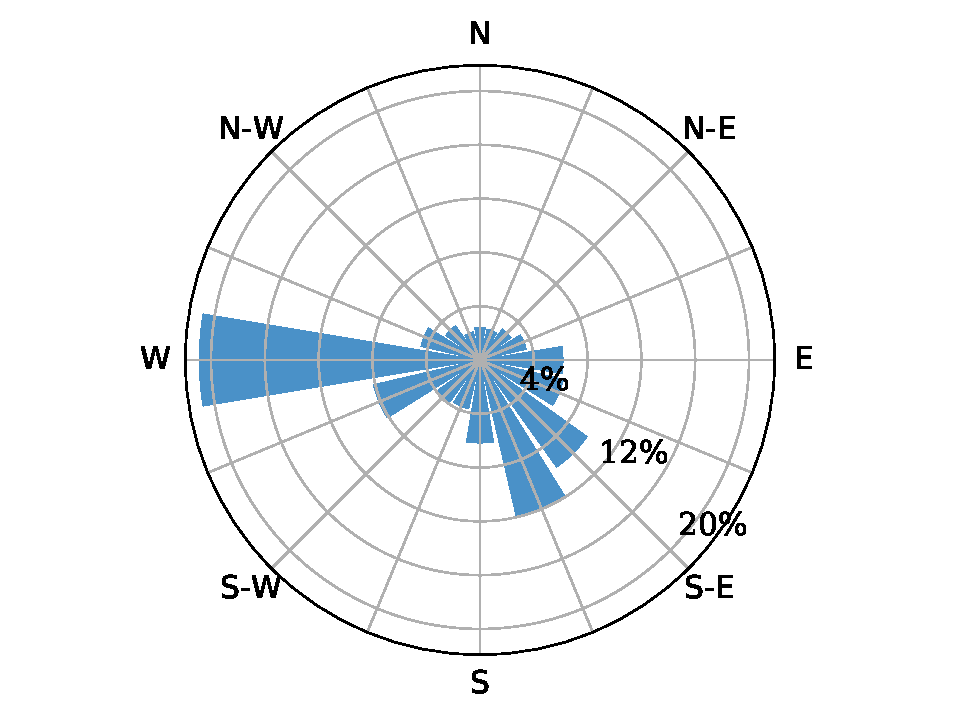
\includegraphics[width=.5\textwidth]{windrose.pdf}
	\caption{The wind frequency distribution; a bi-modal Gaussian distribution as defined in \cref{Eq:freq}}
	\label{Fig:freq}
\end{figure}



\subsection{Participant Results}

We will first present the two case studies described in \cref{Sec:OptOnly,Sec:Cmbnd} at the Torque conference held June 20-22 in Milan, Italy. Beyond the self-selected volunteers we acquire from this announcement, we will recruit further participants through existing communication channels established among participants of the International Energy Association's (IEA's) Task 37 initiative. A similar study as this one has been done through Task 37 regarding turbine rotor aerodynamics, of which this work (applied to wind farms in general) is modelled.

Results will be submitted according to specified formats laid out in the announcement documents. All submissions will be in a compressed \texttt{.zip} file, containing:

\begin{enumerate}
	\item A \texttt{.pdf} of the method/process description
	\item A \texttt{.txt} file with the quantitative optimization results
\end{enumerate}

The \texttt{.pdf} document will contain the below information for the Combined Case Study. For the Optimization Only Case Study, wake model information will not apply.

\begin{itemize}
	\item Wake Model
	      \begin{itemize}
		      \item Model name
		      \item Governing wake equations (if possible)
		      \item Description of general model shape (i.e.~smooth, flat, Gaussian curve, presence of discontinuities, etc.)
		      \item What factors are accounted for by your model (i.e.~partial wake, shear, turbulence, etc.)
		      \item Paper citation for description of model (if applicable)
		      \item Other relevant wake model details
	      \end{itemize}
	\item Optimization algorithm (including version and any non-default settings or modifications)
	      \begin{itemize}
		      \item Name of algorithm
		      \item General type of algorithm (e.g. gradient-free, gradient-based)
		      \item Specific algorithm type (e.g. particle-swarm, genetic-algorithm, sequential quadratic programming, etc)
		      \item If you used a gradient-based method, how did you obtain the gradients.
		      \item Number of AEP function calls
		      \item Programming language(s) utilized
		      \item Other relevant algorithm details
	      \end{itemize}
	\item Computer hardware specifications
	      \begin{itemize}
		      \item Manufacturer/Model/Speed of processor (GHz)
		      \item Number of cores utilized
		      \item System total RAM
	      \end{itemize}
	\item How you decided on the starting turbine locations for your final optimized results
	\item Time required for optimization convergence
	\item Links to relevant code(s) (if possible)
	\item Other details you consider relevant
	\item Bibliography
\end{itemize}

The text file will contain two sections: 1) for the baseline, optimized baseline, initial, and  optimal AEP values and 2) for the turbine numbers and their corresponding optimized baseline, initial and optimized $x$ and $y$ locations.




\begin{centering}
	\section{Preliminary Results}
\end{centering}

\subsubsection{Optimization Only Case Study}

Preliminary results with a single gradient-based optimizer (Sparse Nonlinear OPTimizer, SNOPT) and a gradient-free method (Augmented Lagrangian Particle Swarm Optimizer, ALPSO's) are given in \cref{tab:OptOnlyPrelim}.

\begin{table}[]
	\begin{center}
		\begin{tabular}{|l|p{1.7cm}|p{2cm}|l|}
			%{ |p{3cm}|p{3cm}|p{3cm}|p{3cm}|  }
			\hline
			Optimizer & Number of Turbines & Optimal AEP (MWh$*10^6$) & Time to Run \\
			\hline
			\hline
			SNOPT     & 16                 & 1.09957                  & 3m          \\
			          & 36                 & 2.35432                  & 20m         \\
			          & 64                 & 4.11459                  & 2h 56m 23s  \\
			\hline
			ALPSO     & 16                 & 1.10784                  & 10m 27s     \\
			          & 36                 & 2.23475                  & 2h 56m 53s  \\
			          & 64                 & 4.01433                  & 8h 32m 36s  \\
			\hline
		\end{tabular}
	\end{center}
	\caption{Preliminary results with a single gradient-based and gradient free optimization}
	\label{tab:OptOnlyPrelim}
\end{table}

Preliminary results are in line with current knowledge, that gradient-based methods, in general, are much quicker than gradient-free. Though it is interesting that the time savings does not continue to diverge with increased wind farm size, since preliminary results show that the difference in solution time actually draws closer together when moving from the 36 to the 64 turbine cases. More results will be needed to see if this convergence of time savings also occurs under other implementations of gradient-based and gradient-free methods.

Another interesting data point that will be further investigated is that in the smallest scenario (the 16 turbine wind farm), the gradient-free method comes to an optimum AEP that is slightly better (by $0.75\%$),  though by taking about $\sim30\%$ longer to converge. This superior solution may be due to the improved ability of gradient-free methods to escape local mimima, but more data will be needed to see if this is a trend, since the other two wind farm sizes saw the gradient-based method with superior AEP values.

The SNOPT preliminary optimal turbine arrangements depicted in \cref{fig:SNOPTLayouts} show a general trend of turbine placement along rows perpendicular to the major axes of the wind frequency distribution. Though a few individual turbine exceptions exist, their placement out of line with these rows is probably more due to a local minima resulting from the random start, than discovery of a globally superior location. Further optimizations will be run with turbines manually placed along these lines in order to achieve an even higher optimum AEP convergence.

\begin{figure}[H]
	\centering
	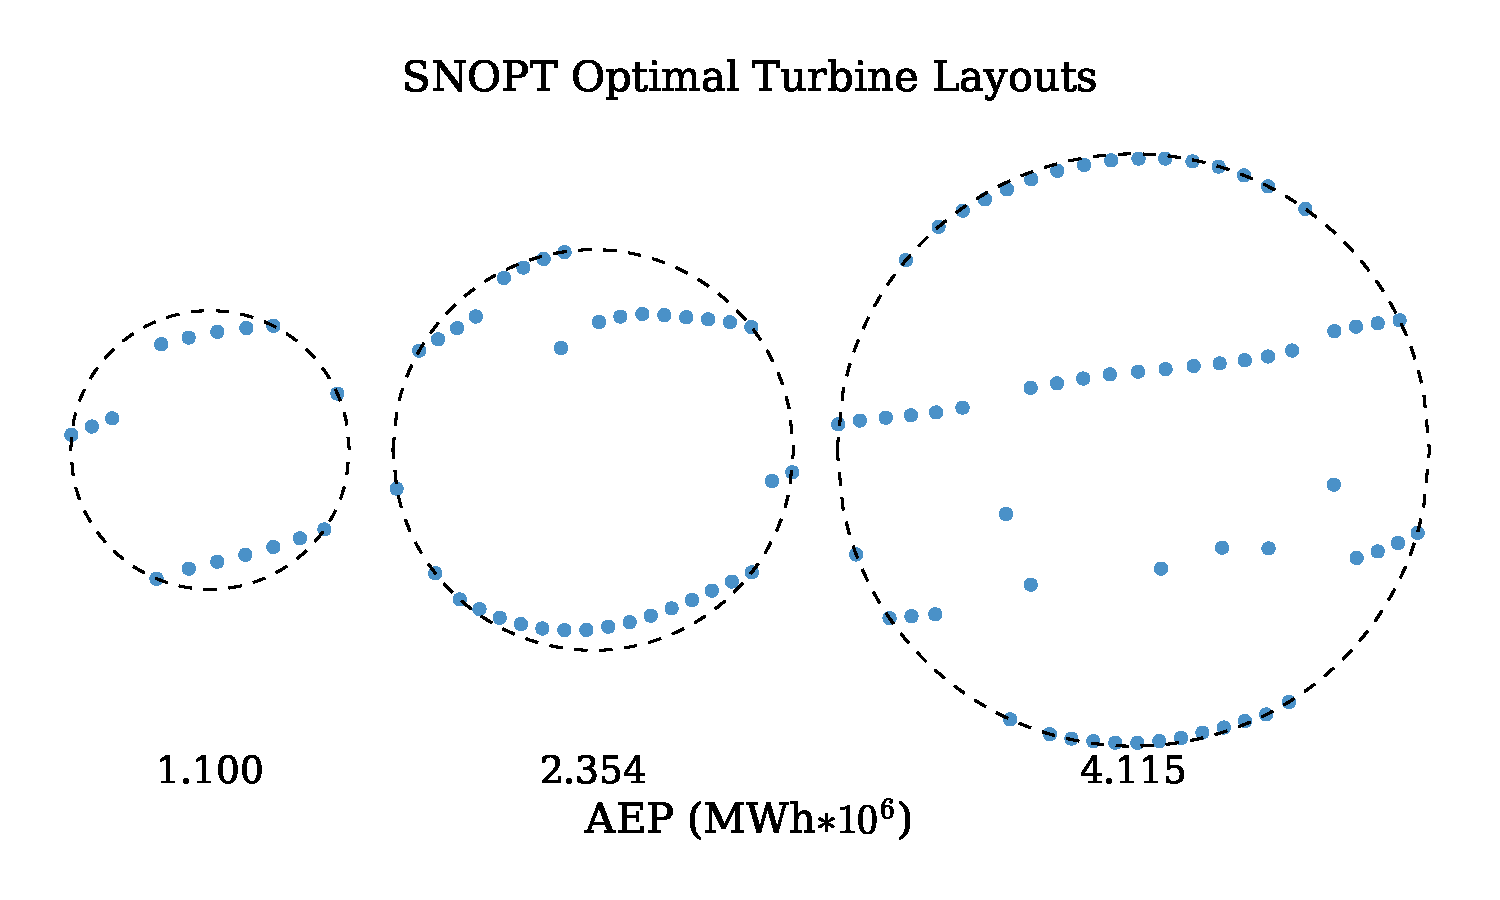
\includegraphics[width=\textwidth]{SNOPTlayouts.pdf}
	\caption{Optimized Layouts for 16, 36, and 64 turbine wind farms}
	\label{fig:SNOPTLayouts}
\end{figure}

\subsubsection{Combined Physics Model/Optimization Algorithm Case Study}

Preliminary results for the second case study show quite intuitive placement for the Simplified Gaussian wake model (\cref{fig:GaussianCombined}), and not as intuitive placement for the FLORIS wake model (\cref{fig:FLORISCombined}).

The Gaussian model placed as many turbines perpendicular to the major axis of wind frequency distribution, while not violating the 2 diameter minimum spacing constraint. The single turbine left was then pushed as far from the others as possible.

The FLORIS model placement found a layout which permits turbines to be unobstructed along the major axis of wind direction in the North-South direction, though does not seem to follow a pattern for relative placement within these lanes. Both the Simplified Bastankhah and FLORIS implememntations for this case study used the same SNOPT optimizer, so differences must lie within the interaction with the wake model characteristics. More participants with differing wake models will be required to see if either one of these layouts is indicative of a trend.

\begin{figure}[H]%
	\centering
	\subfigure[]{%
		\label{fig:GaussianCombined}%
		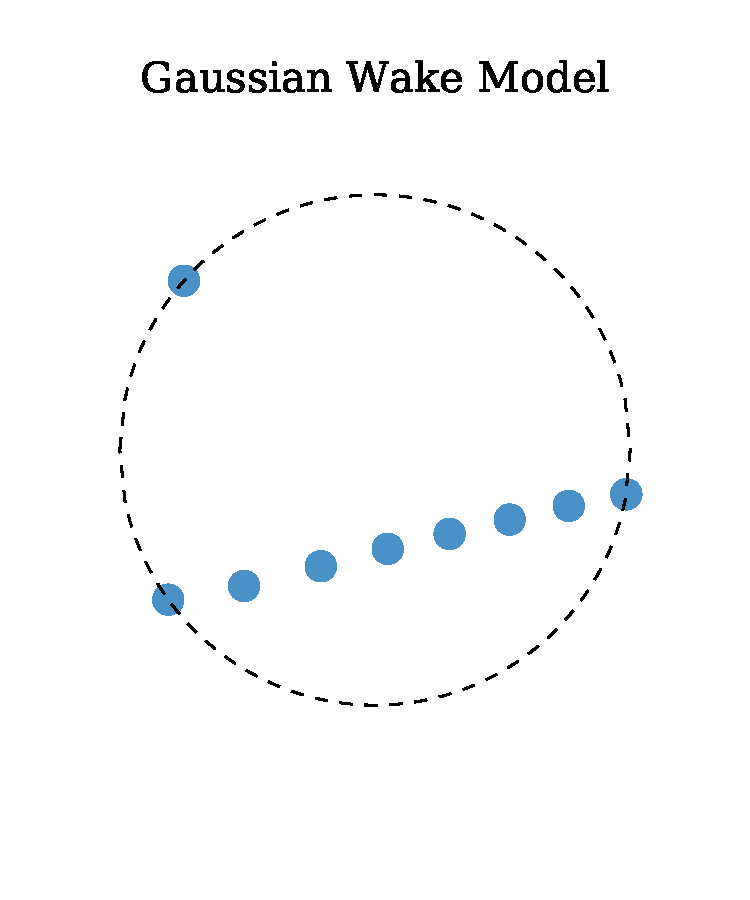
\includegraphics[width=.3\textwidth]{GaussianLayout.pdf}}%
	\qquad
	\subfigure[]{%
		\label{fig:FLORISCombined}%
		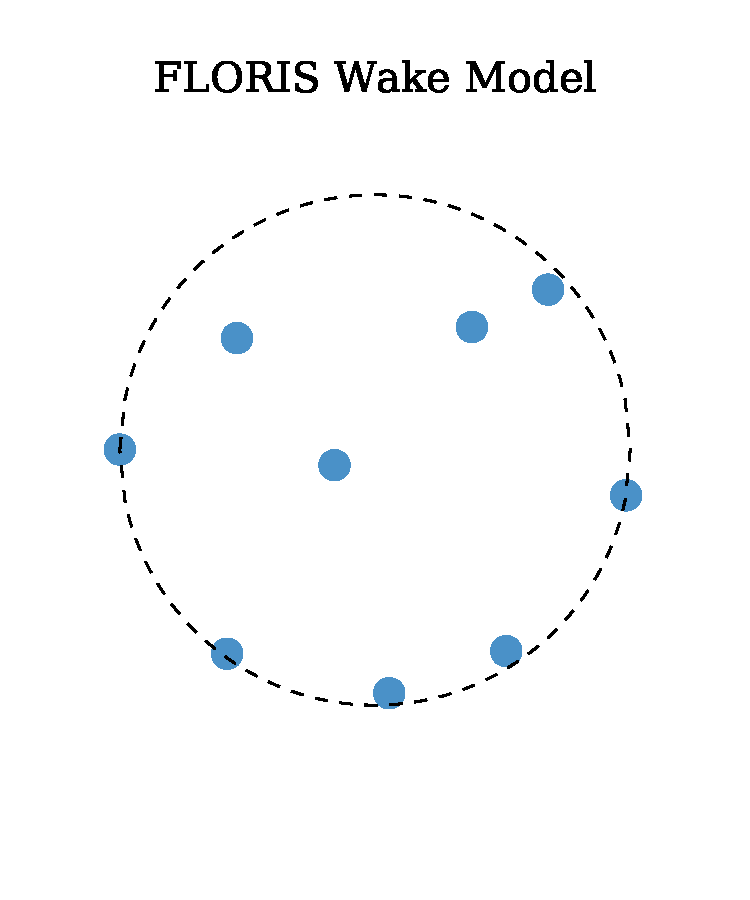
\includegraphics[width=.3\textwidth]{FLORISLayout.pdf}}%
	\caption{Comparison of optimized results of the Simplified Bastankhah's Gaussian wake model with the FLORIS wake model, both optimized with SNOPT}
\end{figure}
Due to time constraints, LES comparisons of the two layouts have not yet been completed. Though if self-reported AEP is to be trusted, the Simplified Bastankhah Model with near-linear turbine placement is the far superior of the two. More time will be needed to make the comparative decision regarding the LES-reported AEP between these two wake models.

\bigskip
\begin{centering}
	\section{Conclusion and Continued Development}
\end{centering}
\subsection{Conclusions}
The preliminary participant results indicate a superiority of gradient-free methods, and therefore wake models that can supply gradients will tend to give quicker and better results. However, within the small sample size observed, the gradient-free method found a superior AEP placement in the smallest wind farm scenario, despite requiring more time for convergence. More participant results are needed, but from this preliminary it appears that in smaller wind farm scenarios, if convergence time is not a constraint, gradient-free methods may tend to provide superior results.

As the farm size increased from 36 to 64 turbines, the disparity of convergence time between gradient-based and gradient-free methods lessened. More participant implementations and results are needed to see if this is a trend or an anomaly.

We expect that an increased sample size of EWMs will more clearly show the trends between gradient-based and gradient-free methods. From preliminary data, it seems that for highly directional wind roses, the optimized trend is for linear turbine placement along lines perpendicular to the major axis of wind frequency direction.

\subsection{Continued Development}
To continue work on with this study, we will need more participant data of both gradient-based and gradient-free methods. This will reveal if gradient-free methods truly tend to be superior for the smaller wind farm scenarios, and if required convergence time for large farm scenarios approach comparability.

Further improvement will be to review and improve the initial turbine locations in the Optimization Only Case Study. For preliminary results, only random starts were used. Warm starts, as well as human-intuitive starts based on the results from random starts will be attempted, in order to obtain higher optimal AEP values.

A large alteration we will explore is changing the wind direction frequency to one that is more omni-directional. Preliminary results show that the given bi-directional wind frequency (simulating a canyon) simply pushes turbines into rows perpendicular to the major axis of wind direction. However an omni-directional frequency may not give results more or less interesting than the bi-directional wind frequency used, simply practices more useful in geographic scenarios of that type, such as applications offshore.

Another small alteration we may explore is constraining the Combined Case Study's wind farm size to force optimal designs other than a single linear row. Using the NREL 5MW reference turbine, with a constant rotor diameter of 126.4 meters, a farm diameter of 2200 m permits side-by side placement of up to 8 turbines while maintaining the minimum 2-turbine distance constraint. We will explore either expanding the minimum distance constraint, or decreasing the wind farm radius, to see if more interesting results are delivered.

%To improve the optimization, we will include the von Mises stress as a constraint. In past research, in which the tower height varied but rotor diameter was not a design variable, we observed that the von Mises stress constraint was never active, leading us to remove it from the optimization. This may not hold true when rotor diameter is allowed to vary, and will be important to check.

%Finally, we will optimize from many different starting points because the design space to this problem is highly multi modal. One way to overcome this is to use a gradient free algorithm. Unfortunately this would limit us to a relatively small number of design variables because of computational expense required for large gradient free problems. We will overcome the multi modality of this problem by using a lot of random starting points to find the best solution possible. 

As preliminary results show in \cref{fig:SNOPTLayouts}, many local optima exist in these scenarios. For this reason, we believe that either a great deal of human intuition on starting locations will be needed, or unique optimization strategies and algorithms will be required to find turbine locations that result in superior AEP results. We are confident that this study will result in improved recommendations for WFLO researchers on best practices in EWM and optimization algorithm selection strategies.

Finally all preliminary results are suspect due to the smallness of the sample size. More participant data is needed to determine of the results thus-far seen are anachronistic, or signs of a larger trends.

\pagebreak
\bibliographystyle{aiaa}
\bibliography{references}
\end{document}